
\documentclass [12pt, a4paper]{report}
\usepackage[left=2cm, right=2cm, top=2.5cm, bottom=3.5cm, bindingoffset=0cm]{geometry}
\usepackage[english]{babel}
\usepackage{fontspec} 
\setmainfont{Arial}
\usepackage{float}
\usepackage{caption}
\captionsetup[table]{position=above,justification=raggedright}
%\captionsetup[figure]{}
\usepackage{tikz}
\usepgflibrary{fpu}
\usepackage{pgfplots}
\usepackage{pgfplotstable}
\pgfplotsset{compat=1.5}

\usepackage{amssymb}
\usepackage{titlesec} %настройка шрифтов оглавлений

\titleformat{\section}{\normalfont\large\bfseries}{\thesection}{1em}{}
\titleformat{\subsection}{\normalfont\normalsize\bfseries}{\thesubsection}{1em}{}

\setlength{\arrayrulewidth}{1pt}%установка ширины линий таблиц

\usepackage{color,colortbl}
\usepackage{color,xcolor}
\usepackage{array}
\usepackage{tabularx}
\usepackage{longtable}
\extrarowheight = 2pt %добавление пространства под верхней линейкой таблицы


\usepackage{graphicx}
\usepackage{multirow}%для возможности объединения строк в таблицах

\usetikzlibrary{plotmarks}

\usepackage[ddmmyyyy]{datetime}
\renewcommand{\dateseparator}{.} 

\usepackage{textcomp} %для добавления знака копирайта
\usepackage{fancyhdr}
\pagestyle{fancy}

\usepackage{lastpage}

\usepackage{ragged2e}
\newcommand{\jj}{\righthyphenmin=20 \justifying} %команда для выравнивания текста по ширине


\headheight = 103pt
\headsep = 8pt
\footskip = 1cm
%\textheight = 21.5cm
\textheight = 22.5cm
\fancyhf{}  % убираем текущие установки для колонтитулов
\renewcommand{\headrulewidth}{0.0pt}
\fancyhead[C]{
\begin{tabularx}{\textwidth}{|>{\raggedright}X|l|l|}
\multicolumn{3}{l}{\large{\TECH\ \MOS\ \CHIPID\ DTC Test Report ~---\ \version ~---\ \today}} \\
\hline
Chip ID: \CHIPID & MPW ID: \MPWID & Wafer No.: \WAFERNO \\
\hline
Batch ID: \BATCHID & Lot ID: \LOTID & Dies: \DIES \\
\hline 
\multicolumn{2}{|l|}{Core lib.: \CORELIBRARY} & IO lib.: \IOLIBRARY \\
\hline
\multicolumn{3}{|l|}{Process: \PROCESS} \\
\hline
\end{tabularx}
}
\fancyfoot[C]{\footnotesize \thepage /\footnotesize \pageref{LastPage}}
\fancyfoot[L]{\footnotesize{\today \ \textcopyright \  X-FAB Semiconductor Foundries}}
\fancyfoot[R]{\footnotesize{\version}}


\fancypagestyle{plain}{
\fancyhf{}  % убираем текущие установки для колонтитулов
\renewcommand{\headrulewidth}{0.0pt}
\fancyhead[C]{
\begin{tabularx}{\textwidth}{|>{\raggedright}X|l|l|}
\multicolumn{3}{l}{\large{\TECH\ \MOS\ \CHIPID\ DTC Test Report ~---\ \version ~---\ \today}} \\
\hline
Chip ID: \CHIPID & MPW ID: \MPWID & Wafer No.: \WAFERNO \\
\hline
Batch ID: \BATCHID & Lot ID: \LOTID & Dies: \DIES \\
\hline 
\multicolumn{2}{|l|}{Core lib.: \CORELIBRARY} & IO lib.: \IOLIBRARY \\
\hline
\multicolumn{3}{|l|}{Process: \PROCESS} \\
\hline
\end{tabularx}
}
\fancyfoot[C]{\footnotesize \thepage /\footnotesize \pageref{LastPage}}
\fancyfoot[L]{\footnotesize{\today \ \textcopyright \  X-FAB Semiconductor Foundries}}
\fancyfoot[R]{\footnotesize{\version}}
}

\usepackage{etoc}
\renewcommand{\etocaftertitlehook}{\pagestyle{plain}}
\renewcommand{\etocaftertochook}{\thispagestyle{plain}}

\setcounter{secnumdepth}{5}
\setcounter{tocdepth}{5}

\usepackage{titletoc}
\usepackage[hidelinks, breaklinks]{hyperref} 
\usepackage{tocloft} 
\dottedcontents{chapter}[1.6em]{}{1.6em}{1pc}
%Изменение стиля страницы с оглавлением.%%%%%%%%%%%%%%%
\setlength{\cftbeforetoctitleskip}{0pt} % отступ перед оглавлением
\setlength{\cftaftertoctitleskip}{0pt} % отступ после оглавления

%Оформление вывода заголовков Chapter%%%%%%%%%%%%%%
\makeatletter
\def\thickhrulefill{\leavevmode \leaders \hrule height 1ex \hfill \kern \z@}
\def\@makechapterhead#1{%
  {\parindent \z@ 
        \reset@font\Large\bfseries
        \begin{tabular}{p{6mm}p{25cm}}
          {\thechapter{}}
          &
          \Large #1
        \end{tabular}
        \par\nobreak
    \vskip 10\p@ %расстояние от названия главы до текста
  }}
%%%%%%%%%%%%%%%%%%%%%%%%%%%%%%%%%%%

%для выравнивания названий таблиц по левому краю%%%%%%%%%%%%%%%%%%%%%%
\newcommand{\@maketablecaption}[2]{
    \vskip\abovecaptionskip
    \sbox\@tempboxa{#1 --- #2}%
    \ifdim \wd\@tempboxa >\hsize
        #1 --- #2\par
    \else
        \global \@minipageFailse
        \hb@xt@\hsize{\box\@tempboxa}%
    \fi
    \vskip\belowcaptionskip}
\renewcommand{\table}{\let\@makecaption\@maketablecaption\@float{table}}
%%%%%%%%%%%%%%%%%%%%%%%%%%%%%%%%%%%%%%%%%%%%%%%
%DTC_Config
\graphicspath{{images/}}
\newcommand{\TECH}{$Tech$}
\newcommand{\MOS}{$MOS$}
\newcommand{\IOMODELS}{$IOModels$}
\newcommand{\MEMORYMODELS}{$MemoryModels$}

\newcommand{\CHIPID}{$ChipID$}
\newcommand{\MPWID}{$MPWID$}
\newcommand{\BATCHID}{$BatchID$}
\newcommand{\LOTID}{$LotID$}
\newcommand{\CORELIBRARY}{$CoreLib$}
\newcommand{\IOLIBRARY}{$IOLib$} 
\newcommand{\PROCESS}{$Process$}
\newcommand{\WAFERNO}{$Wafer$}
\newcommand{\TESTTYPE}{$TestType$}
\newcommand{\PACKAGING}{$Packaging$}
\newcommand{\DIES}{$Dies$}
\newcommand{\AUTHOR}{$Author$}
\newcommand{\EMAIL}{$Email$}
\newcommand{\MEASURED}{$Measured$}
\newcommand{\version}{$Version$}

\newcommand{ \VDDRPIN}{VDDR\_PAD\_5V}
\newcommand{ \VDDOPIN}{VDDO\_PAD\_5V}
\newcommand{ \VDDPADPIN}{VDD\_PAD\_1\_8V}
\newcommand{ \VDDCOREPIN}{vdd!}
\newcommand{ \VDDSEP}{vdd!\_sep}
\newcommand{\VDDNA}{vdd\_NA2\_NO2}
%\newcommand{\GNDSEP}{RAMGND\_SEP}
%\newcommand{\GNDSEPI}{RAMGND\_SEP1}
\newcommand{\VDDMEMORYIPIN}{VDD\_SPRAMB2KX16}
\newcommand{\VDDMEMORYIIPIN}{VDD\_SPRAMB256X16}
\newcommand{\VDDMEMORYIIIPIN}{VDD\_SPRAM4KX16}
%\newcommand{\VDDMEMORYIVPIN}{\ }

\newcommand{\VDD}{1.8}
\newcommand{\VDIO}{5}
\newcommand{\TEMP}{+25}

\newcommand{\MEMORYI}{XSPRAMBLP2KX16T\_CSB\_1\ }
\newcommand{\MEMORYII}{XSPRAMBLP256X16T\_CSB\_1\ }
\newcommand{\MEMORYIII}{XSPRAML4KX16P\_M32\ }
%\newcommand{\MEMORYIV}{XSPRAMLP\_4096X16P\_M32 }

\newcommand{\CONTACTPASS}{}%%%%%%% NUMBER OF DIES PASSED CONTACT TEST

\newcommand{\testI}{IO test\ }
\newcommand{\testII}{NANDTREE test\ }
\newcommand{\testIII}{LOGIC\_ATPG\ }
\newcommand{\testIV}{LOGIC\_PART\_NSCAN\ }
\newcommand{\testV}{LIFE\_PART\ }
\newcommand{\testVI}{\MEMORYI data/control logic\ }
\newcommand{\testVII}{\MEMORYII data/control logic\ }
\newcommand{\testVIII}{\MEMORYIII data/control logic\ }
\newcommand{\testIX}{\MEMORYI March C-\ }
\newcommand{\testX}{\MEMORYII March C-\ }
\newcommand{\testXI}{\MEMORYIII March C-\ }
\newcommand{\testXII}{\MEMORYI Data retention\ }
\newcommand{\testXIII}{\MEMORYII Data retention\ }
\newcommand{\testXIV}{\MEMORYIII Data retention\ }
\newcommand{\testXV}{\MEMORYI Data retention in LSM\ }
\newcommand{\testXVI}{\MEMORYII Data retention in LSM\ }
\newcommand{\testXVII}{}
\newcommand{\testXVIII}{}
\newcommand{\testXIX}{}
\newcommand{\testXX}{}

%%%%%%%%%%%%%%%%%%%%%%%%%%%%%%%%%%%%%%%%%%%%%%


% COLORS

\definecolor{darkishgreen}{RGB}{39,203,22}
\definecolor{LightCyan}{rgb}{0.88,1,1}
\definecolor{Gray}{gray}{0.9}
\definecolor{lightRed}{RGB}{230,170,150}
\definecolor{modRed}{RGB}{230,82,90}
\definecolor{Red}{RGB}{230,6,6}
\definecolor{Green}{RGB}{0,255,0}
\definecolor{darkGreen}{RGB}{0,192,0}
\definecolor{BIN0}{RGB}{0,192,0}
\definecolor{BIN1}{RGB}{0,255,0}
\definecolor{BIN2}{RGB}{255,255,0}
\definecolor{BIN3}{RGB}{224,160,0}
\definecolor{BIN4}{RGB}{224,96,0}
\definecolor{BIN5}{RGB}{255,0,0}
\definecolor{NoData}{RGB}{192,192,192}


% LEGENDS
\newcommand{\ratelegend}{VDD=\VDD V; VDIO=\VDIO V; T=+25$^{\circ}$C; Rate=1000ns}  
\newcommand{\ratelegendret}{VDIG=\VDD V; VDIO=\VDIO V; T=+25$^{\circ}$C; Rate=1000ns}  
\newcommand{\ratepercentlegend}{VDD=\VDD V $\pm$ 10\%; VDIO=\VDIO V; T=+25$^{\circ}$C; Rate=1000ns}  
\newcommand{\noratelegend}{VDD=\VDD V; VDIO=\VDIO V; T=+25$^{\circ}$C}  
\newcommand{\vworklegend}{VDIO=\VDIO V; T=+25$^{\circ}$C; Rate=1000ns}  
\newcommand{\dataretlegend}{VDIG=\VDD V; VDIO=\VDIO V; T=+25$^{\circ}$C; Rate=1000ns} 
\newcommand{\ramgndlegend}{VDD=\VDD V; VDIO=\VDIO V; T=+25$^{\circ}$C; Rate=1000ns} 

% - Легенда для Data retention wafer map%%%%%%%%%%%%%%%%%%%%%%%%%%%%%%%%
\newcommand{\mylegendret}{\scriptsize{$\square$ Bad contact \ \ \textcolor{Red}{$\blacksquare$} Functional FAIL \ \ \textcolor{Green}{$\blacksquare$}     
Functional PASS, VRAM: OK ~\\ \textcolor{BIN4}{$\blacksquare$} Functional PASS, VRAM>Simulated value}}
%%%%%%%%%%%%%%%%%%%%%%%%%%%%%%%%%%%%%%%%%%%%%

% - Легенда для IDDQ wafer map%%%%%%%%%%%%%%%%%%%%%%%%%%%%%%%%
\newcommand{\myIDDQlegend}{\scriptsize{$\square$ Bad contact \ \ \textcolor{BIN0}{$\blacksquare$}     
IDDQ<TM \textcolor{BIN1}{$\blacksquare$} TM<IDDQ<WP \\ \textcolor{BIN2}{$\blacksquare$} WP<IDDQ<10*WP \ \ \textcolor{BIN3}{$\blacksquare$} 10*WP<IDDQ<100*WP 
\\ \textcolor{BIN4}{$\blacksquare$} 100*WP<IDDQ<1000*WP  \ \ \textcolor{BIN5}{$\blacksquare$} IDDQ>1000*WP}}

% - Легенда для wafer map%%%%%%%%%%%%%%%%%%%%%%%%%%%%%%%%
\newcommand{\mylegend}{\scriptsize{$\square$ Data test FAIL \ \ \textcolor{Green}{$\blacksquare$}     
Functional PASS \ \ \textcolor{Red}{$\blacksquare$} Functional FAIL}}
% LEGENDS




\begin{document}

%Title_Page

~\\
~\\
\center{
\includegraphics[scale=1.05]{xfab_logo.png}}
~\\
~\\
~\\
~\\

\center{ \Huge\textbf{DTC \CHIPID\ Test Report}
\large
~\\
~\\
~\\
  
\begin{tabular}{p{4cm}p{10.0cm}}
Chip ID:  & \CHIPID \\ 
MPW ID: & \MPWID \\
Batch ID: & \BATCHID \\
Lot ID: & \LOTID \\ 
Process: & \PROCESS \\
IO library: & \IOLIBRARY\\
Core library: & \CORELIBRARY \\
Packaging: & \PACKAGING \\
Type: & \TESTTYPE Test \\
Wafer No.: & \WAFERNO \\
Number of dies: & \DIES \\
Author: & \AUTHOR \\
Email: & \EMAIL \\
Measurement: & \MEASURED \\
Date: & \today \\
Version: & \version \\
\end{tabular}



%Version_Page
\newpage
\raggedright
\Large {\bf Version History}
\center{
\normalsize
%\begin{tabular}{|p{1.86cm}|p{2.37cm}|p{7.73cm}|p{4.29cm}|}
\begin{tabularx}{\textwidth}{|l|l|X|l|}
\hline
%\rowcolor{Gray}
 Version  &  Date &   Description &  Author  \\ 
\hline
 \version & \today & Initial version & Alexander Krylov \\
\hline
\end{tabularx}
}
\normalsize

\newpage
\raggedright
\tableofcontents
\newpage
\pagestyle{fancy}
\fancypagestyle{plain}

\chapter{DTC description}

Please refer to:
\begin{itemize}
%Start DTC description
%End DTC description
\end{itemize}

%%%%%%%%%%%%%%%%%%%%%%%%%%%%%%%%%%%%%%%%%%%%%%%%%%%%%%%%%%%%
\jj
\newpage
\section{Supply pins}

 \vskip -5mm
\begin{table}[htbp]
\captionof{DTC  \CHIPID\ power supply pins.}
\label{tabular:pins} 
\begin{center}
\vskip 5mm
\begin{tabularx}{\textwidth}{|r|r|X|}
\hline
Pin No. & Supply name & Description \\ \hline
%Start supply pins
%End supply pins 


\end{tabularx}
\end{center}
\end{table}



 \vskip -5mm
\begin{table}[htbp]
\begin{center}
\caption{ \label{pingroups}Supply pin groups.} 
~\\
\begin{tabularx}{\textwidth}{|l|X|}
\hline
 VDD: & VRAM, VDIG \\
\hline
%VRAM: & \VDDMEMORYIVPIN \\
%\hline
VRAM: & \VDDMEMORYIPIN, \VDDMEMORYIIPIN, \VDDMEMORYIIIPIN \\
\hline
VDIG: & \VDDCOREPIN, \VDDPADPIN, \VDDSEP, \VDDNA \\
\hline
VDIO:& \VDDOPIN, \VDDRPIN \\
\hline
%VGND:& \GNDSEP \\
%\hline
\end{tabularx}
\end{center}

\end{table}

%%%%%%%%%%%%%%%%%%%%%%%%%%%%%%%%%%%%%%%%%%%%%%%%%%%%%%%%%%%%

\newpage
\section{Bonding diagram}

\vskip -5mm
\begin{figure}[h!]
%\caption{\bf DTC top level block diagram:}
\caption{ Bonding diagram \CHIPID}
\vskip -7mm
\label{toplevel}
\center{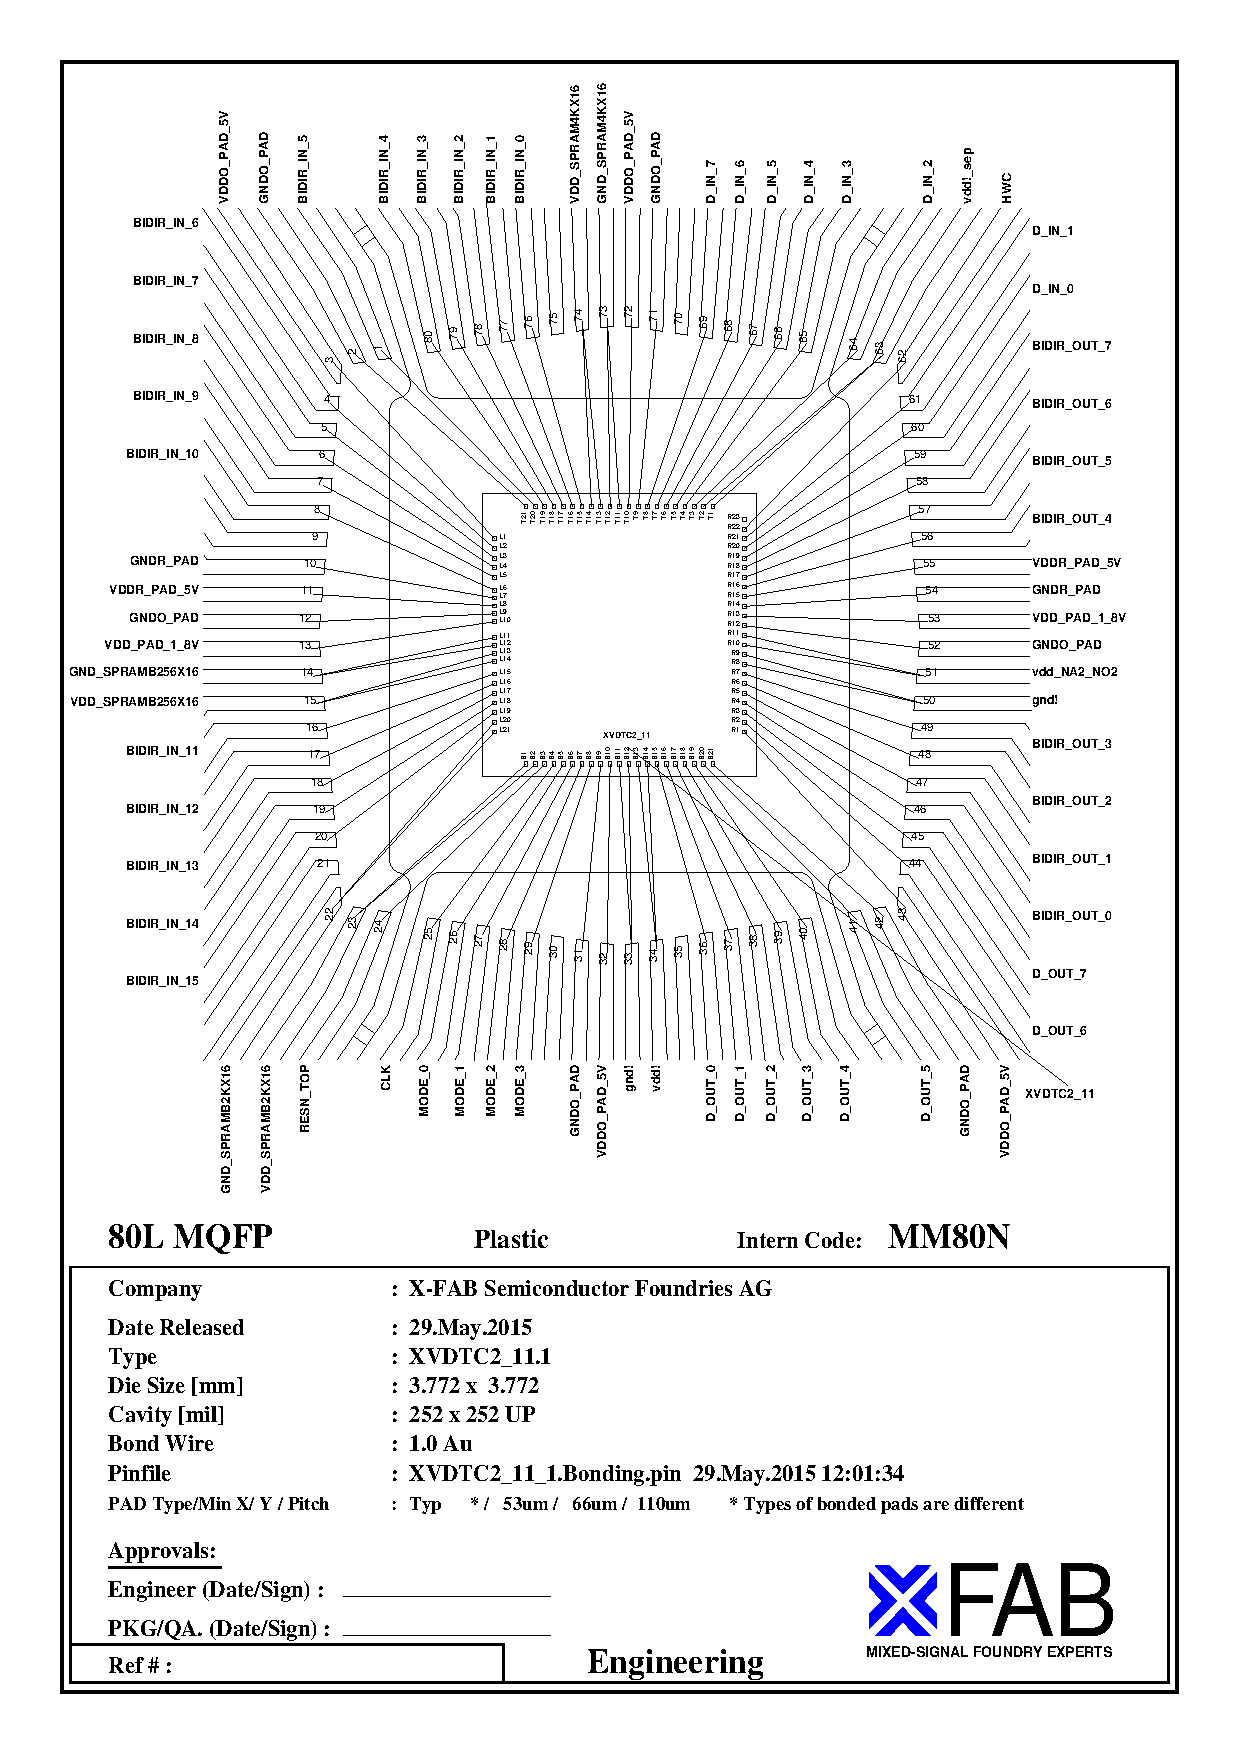
\includegraphics[scale=0.67]{bonding.pdf}} %%%%%%%%%% BONDING
\end{figure}

%%%%%%%%%%%%%%%%%%%%%%%%%%%%%%%%%%%%%%%%%%%%%%%%%%%%%%%%%%%%

\chapter{Test description}

%\vskip -5pt
\section{Test patterns}

Please refer to:
\begin{itemize}
%Start test patterns
%End test patterns
\end{itemize}


%%%%%%%%%%%%%%%%%%%%%%%%%%%%%%%%%%%%%%%%%%%%%%%%%%%%%%%%%%%%

\section{Test hardware}

\begin{itemize}
\item Semi-automatic wafer prober Suss MicroTec PA200
\item Modular test system Konrad Technologies FINN-7500 equipped with IMMS PMU32, Konrad Technologies DIG50IO, and three High Speed Digital IO PXI-6552 plug-in cards. 
\item Probe card HTT “SSMB96” Rev. 3.1 and the needle carrier “DTC\_018”.
%\item Digital oscilloscope Agilent DSO6104A.
\end{itemize}

\section{Test software}
\begin{itemize}
\item Main DTC test program: “\CHIPID.vi” rev.1.0
\item Program for creating patterns: “IORead.vi” rev.6.3 
\end{itemize}

%%%%%%%%%%%%%%%%%%%%%%%%%%%%%%%%%%%%%%%%%%%%%%%%%%%%%%%%%%%%

\section{Color meaning in tables}

Green text means that measured values are inside the simulation range and red means that they are outside. 


%%%%%%%%%%%%%%%%%%%%%%%%%%%%%%%%%%%%%%%%%%%%%%%%%%%%%%%%%%%%


\chapter{Functional test}

%ПРОБЛЕМЫ С IO ЯЧЕЙКАМИ
\renewcommand{\VDIO}{3.3}
\textcolor{red}{Problems with IO cells. Functionality measured with VDIO=3.3V.}
%ПРОБЛЕМЫ С IO ЯЧЕЙКАМИ

\input{funk_1.62.tex}
\newpage
\input{funk_1.8.tex}
\newpage
\input{funk_1.98.tex}
\newpage

%ПРОБЛЕМЫ С IO ЯЧЕЙКАМИ
\renewcommand{\VDIO}{5}
%ПРОБЛЕМЫ С IO ЯЧЕЙКАМИ

%%%%%%%%%%%%%%%%%%%%%%%%%%%%%%%%%%%%%%%%%%%%%%%%%%%%%%%%%%%%

\chapter{Parameter test: IDDQ}

\input{yield.tex}
 
\newpage 
\section{IDDQ IO block}
\input{o.tex}

\newpage
\input{r.tex}

\newpage
\input{p.tex}


\newpage
\section{IDDQ Core logic block}
\input{na2ab.tex}

\newpage
\input{na2!a!b.tex}

\newpage
\input{vsep.tex}

\newpage
\input{v.tex}


\newpage
\section{IDDQ memory block}
\input{2k.tex}

\newpage
\input{2klsm.tex}

\newpage
\input{256.tex}

\newpage
\input{256lsm.tex}

\newpage
\input{4k.tex}

\newpage
\input{voltages.tex}

%ПРОБЛЕМЫ С IO ЯЧЕЙКАМИ
\renewcommand{\VDIO}{5}
%ПРОБЛЕМЫ С IO ЯЧЕЙКАМИ


%\input{VOLTAGES.tex}
\newpage
\input{procmon.tex}

\newpage
\input{procmonhd.tex}

%%%%%%%%%%%%%%%%

\end {document}
